\documentclass{article}
\usepackage[utf8]{inputenc}
\usepackage{listings}
\usepackage{xcolor}
\usepackage{hyperref}
\usepackage{geometry}
\usepackage{tikz}
\usepackage{float}
\usetikzlibrary{positioning, arrows.meta, shapes.geometric}

\usepackage{listings}

\hypersetup{
    colorlinks=true,
    linkcolor=blue,
    filecolor=magenta,      
    urlcolor=cyan,
    pdftitle={Overleaf Example},
    pdfpagemode=FullScreen,
    }

\urlstyle{same}

\lstset{
  basicstyle=\ttfamily,
  columns=fullflexible,
  breaklines=true,
  postbreak=\mbox{\textcolor{red}{$\hookrightarrow$}\space},
}

% Define colors
\definecolor{codegray}{gray}{0.9}

% Code listing style
\lstdefinestyle{mystyle}{
    backgroundcolor=\color{codegray},   
    commentstyle=\color{green},
    keywordstyle=\color{magenta},
    numberstyle=\tiny\color{codegray},
    stringstyle=\color{purple},
    basicstyle=\ttfamily\footnotesize,
    breakatwhitespace=false,         
    breaklines=true,                 
    captionpos=b,                    
    keepspaces=true,                 
    numbers=left,                    
    numbersep=5pt,                  
    showspaces=false,                
    showstringspaces=false,
    showtabs=false,                  
    tabsize=2
}

\lstdefinelanguage{yaml}{
  keywords={true,false,null,y,n},
  keywordstyle=\color{darkgray}\bfseries,
  basicstyle=\ttfamily,
  sensitive=false,
  comment=[l]{\#},
  commentstyle=\color{purple}\ttfamily,
  stringstyle=\color{red}\ttfamily,
  morestring=[b]',
  morestring=[b]"
}

\lstset{style=mystyle}

\geometry{a4paper,left=20mm,top=20mm,}

\usepackage{makeidx}
\makeindex

\title{Running Applications on Azure Kubernetes Service: A Tutorial}
\author{Shohruh MIRYUSUPOV\thanks{ \href{mailto:shohruh@miryusupov.com}{shohruh@miryusupov.com} }}

\date{\today}

\begin{document}

\maketitle

\begin{abstract}
This tutorial is designed to guide professionals through the intricacies of deploying applications within the Azure Kubernetes Service (AKS) on Windows containers. Adapted to cater to both beginners and seasoned users of Azure or Kubernetes, the tutorial outlines the process of setting up the Azure Container Registry (ACR) for Docker image storage, creating an AKS cluster, and smoothly deploying applications onto this cluster.

The tutorial is structured to ensure ease of understanding and practical application, featuring step-by-step instructions enriched with concrete examples. It utilizes a range of tools and technologies, including Powershell, Docker, Azure CLI (az), Kubernetes command-line tool (kubectl), and YAML configurations, providing a hands-on approach to learning and implementation.

Moreover, the tutorial goes beyond the basics by including appendices that guide users in selecting the most suitable virtual machine for computational needs and choosing appropriate storage options on Microsoft Azure. 

Whether you are looking to deepen your understanding of AKS or seeking practical guidance for your next application deployment on Azure, this tutorial offers the insights and step-by-step procedures to ensure the successful deployment of the solution to the Microsoft Azure Cloud.
\end{abstract}

\includegraphics[scale=.05]{figures/kubernetes-logo.png}
\includegraphics[scale=.07]{figures/docker-logo.jpg}
\includegraphics[scale=.1]{figures/github_actions-logo.png}

\includegraphics[scale=.15]{figures/azure-logo.png}
\includegraphics[scale=.15]{figures/aks-logo.jpg}
\includegraphics[scale=.07]{figures/github-logo.jpg}

\newpage
\tableofcontents

\section*{Introduction}

This tutorial serves as a guide to deploying applications within the AKS. It details the procedure for setting up the ACR to store Docker images, creating an AKS cluster, and deploying an application onto this cluster. The instructions are designed to be straightforward, ensuring even those new to Azure or Kubernetes can follow along and successfully deploy their applications, complete with concrete examples using \texttt{Powershell}, \texttt{docker}, Azure CLI (\texttt{az}), Kubernetes command-line tool (\texttt{kubectl}), and \texttt{YAML} configurations. In Appendix we show how one can find a virtual machine that is appropriate for computational needs and how to select a storage on Microsoft Azure.




\subsection*{Definitions}

In this section we establish the fundamental concepts and terminologies used throughout the tutorial. By defining these terms such as Docker Image, Azure CLI, and AKS Cluster, the tutorial ensures that readers have a shared understanding of the essential elements involved in deploying applications in AKS.

Table \ref{tab:defins} allows to navigate faster navigate, if necessary, through the list of definitions.

\begin{table}[h]
\centering
\begin{tabular}{|p{4cm}|p{4cm}|p{4cm}|}
\hline
\textbf{Docker} & \textbf{Kubernetes} & \textbf{Microsoft Azure} \\ \hline
Docker & Kubernetes & Azure CLI \\
Docker Image & Kubernetes cluster & Azure Container Registry (ACR) \\
Container & Cluster Master & Azure Kubernetes Service (AKS) \\
 & Pods & Azure File Storage \\
 & Deployment & AKS Cluster \\
 & CronJobs & SMB Protocol \\
 & ReplicaSet & Manifest \\
 & Replica &  \\
 & Volume &  \\
 & Persistent Volume (PV) &  \\
 & Persistent Volume Claim (PVC) &  \\
 & Kubelet &  \\
 & Node &  \\ \hline
\end{tabular}
\caption{Definitions grouped by Docker, Kubernetes, and Microsoft Azure}
\label{tab:defins}
\end{table}


\begin{description}
	\item[Docker] \index{Docker} Docker \cite{docker}, \cite{docker_use} is a platform as a service (PaaS) product that uses OS-level virtualization to deliver software in packages called containers. Containers are isolated environments that run applications, ensuring that they work uniformly regardless of the environment. 
    \item[Docker Image] A lightweight, standalone, executable package that includes everything needed to run a piece of software, including the code, runtime, libraries, environment variables, and config files \cite{docker}, \cite{azure}.
 \item[Azure CLI] Azure CLI \cite{azurecli}, \cite{azlist}, short for Azure Command Line Interface, is a set of commands used to manage Azure resources. With Azure CLI, you can interact with Azure services and manage Azure resources such as compute, network, storage, and more. Installation details can be found in \cite{azurecliinstall}. \index{Azure CLI}
    \item[Azure Container Registry (ACR)] A managed Docker container registry service used for storing private Docker container images, similar to Docker Hub, but hosted within Azure for better integration and security with Azure services \cite{azure}. \index{Azure Container Registry} \index{ACR}

    \item[Azure Kubernetes Service (AKS \index{AKS})] A managed container orchestration service, based on Kubernetes, that facilitates deploying, managing, and scaling containerized applications on Microsoft Azure \cite{azure}. Azure Kubernetes Service
    \item[Azure File Storage] A Microsoft Azure service providing cloud file storage via the Server Message Block (SMB) protocol and accessible from anywhere using REST APIs or Azure management tools \cite{azure}. \index{Azure File Storage}

    \item[AKS Cluster] A set of node machines for running containerized applications in AKS. Each AKS cluster includes at least one master machine and multiple worker machines or nodes \cite{azure}. \index{AKS Cluster}
	\item[Kubernetes] Kubernetes is an open-source container orchestration system that automates various aspects of software deployment, scaling, and management \cite{kuber}. A Kubernetes cluster, which is a set of running Linux containers, can be visualized as having two parts: the control plane and the compute machines (or nodes). The control plane manages the state of the cluster, including applications and workloads, while the compute machines actually run these applications. \index{Kubernetes}
	\item[Kubernetes cluster] A Kubernetes cluster consists of a set of worker machines, called nodes, that run containerized applications \cite{kuber}. Every cluster has at least one worker node. The worker node(s) host the Pods that are the components of the application workload. \index{Kubernetes cluster}
	\item[Cluster Master] The Cluster Master \cite{kubmaster} in AKS serves as the brain of the Kubernetes cluster, orchestrating containerized applications' deployment, scaling, and management. It automates the distribution and scheduling of applications across the worker nodes, handles cluster-wide networking, and maintains the overall desired state of the cluster. \index{Cluster Master}
	 \item[Container] A standard unit of software that packages up code and all its dependencies so the application runs quickly and reliably from one computing environment to another \cite{docker}, \cite{azure}. \index{Container}
    \item[Pods] The smallest deployable units of computing that can be created and managed in Kubernetes. A pod encapsulates one or more containers, storage resources, a unique network IP, and options that govern how the container(s) should run \cite{azure}, \cite{kuber}. \index{Pods}

    \item[Execution] The process of running the application within the container, leveraging the resources and environment provided by the container platform \cite{azure}, \cite{kuber}. \index{Execution}
    
    \item[Deployment] In Kubernetes, a Deployment provides declarative updates for Pods and ReplicaSets. You describe a desired state in a Deployment, and the Deployment Controller changes the actual state to the desired state at a controlled rate \cite{azure}. \index{Deployment}
    \item[\texttt{cronjobs}] \texttt{cronjobs} are a Kubernetes resource that allows users to run jobs (i.e., tasks or containers) on a recurring schedule, similar to cron tasks in Unix/Linux systems. A CronJob object specifies a job template and a schedule in the Cron format. Kubernetes then ensures that the jobs are created and executed based on this schedule. CronJobs are useful for automating regular maintenance tasks, running batch jobs, or executing tasks that need to happen at specific times or intervals \cite{azure}, \cite{cronjob}. \index{\texttt{cronjobs}}
    \item[ReplicaSet] A ReplicaSet's purpose is to maintain a stable set of replica Pods running at any given time. It is often used to guarantee the availability of a specified number of identical Pods \cite{azure}, \cite{kuber}. \index{ReplicaSet}
    
    \item[Replica]  A replica \cite{azure}, \cite{kuber} is an instance of a pod, which runs a set of containers. In Kubernetes, a pod represents the smallest deployable unit that can be created, scheduled, and managed. It's often a wrapper for a single container, but it can also contain multiple containers that need to work together. \index{Replica}

    \item[Volume] A directory containing data, accessible to the containers in a pod in Kubernetes, allowing for data persistence and sharing between containers \cite{kuber}. \index{Volume}

    \item[Persistent Volume (PV)] In Kubernetes, a PersistentVolume \cite{kupv} is a piece of storage in the cluster that has been provisioned by an administrator or dynamically provisioned using Storage Classes. It is a resource in the cluster just like a node is a cluster resource. PVs are volume plugins like Volumes, but have a lifecycle independent of any individual Pod that uses the PV. \index{PV} \index{Persistent Volume}

    \item[Persistent Volume Claim (PVC)] A PersistentVolumeClaim \cite{kupv} is a request for storage by a user. It is similar to a Pod. Pods consume node resources and PVCs consume PV resources. Pods can request specific levels of resources (CPU and Memory). Similarly, PVCs can request specific size and access modes (e.g., they can be mounted once read/write or many times read-only). \index{Persistent Volume Claim} \index{PVC}

\item[Kubelet] Kubelet \cite{kubelet} is a fundamental component of Kubernetes, a container orchestration system. It runs on each node in a Kubernetes cluster and has the following responsibilities:
\begin{itemize}
 \item Node registration: it registers the node with the cluster, adding it to the available pool of resources for running workloads.
 \item Pod lifecycle management.
 \item Resource monitoring and reporting.
 \item Executing control plane instructions.
 \item Volume management: it manages the mounting and unmounting of data volumes for pods, allowing for data persistence or sharing between containers within a pod.
 \item Log management. 
\end{itemize} \index{Kubelet}
\item[Node] 
In AKS, a node is essentially a virtual machine (VM) that serves as a worker machine for running containerized applications \cite{kubazure}. These nodes provide necessary resources like CPU, memory, and storage, and are managed by the Kubernetes master. Each node runs the kubelet agent to manage container states based on the master's instructions. Nodes in AKS can vary in size and type, and can be organized into node pools for managing different workloads. While AKS handles node-level operations like scaling, patching, and updating, users are responsible for the applications and containers running on these nodes. \textit{Nodes are the hardware resources that host and run the pods, while pods are logical units that group one or more containers together, sharing specific resources like storage and networking}.

\item[SMB Protocol] SMB \cite{smb}, \cite{smbprotocol}, which stands for Server Message Block, is a network communication protocol used for providing shared access to files, printers, and serial ports among nodes on a network. Initially developed by IBM, it was popularized by Microsoft as it became the standard protocol for file and print sharing in Windows operating systems.
\item[Manifest] A manifest \cite{kubazure} in the context of computing, specifically within Kubernetes, is a YAML (Yet Another Markup Language) file that defines the desired state of an object that the user wants to create on a Kubernetes cluster, such as pods, services, and volume claims. \index{SMB}

\item{\texttt{SSH keys}} \texttt{SSH keys} are a pair of cryptographic keys that can be used to authenticate to an SSH server as an alternative to password-based logins. An SSH key pair consists of a private key and a public key. Private Key  is kept secret and secure by the user. It is used to decrypt data sent to it that has been encrypted with the public key. On the other hand, public key can be shared with anyone and is used to encrypt data before it is sent to the private key holder. \index{\texttt{SSH keys}}
\end{description}

\subsection*{Focus on Clusters and Nodes} \index{Clusters} \index{Nodes}
Figure \ref{fig:aks_node0} shows the structure of Kubernetes cluster and the relationship between the Cluster Master and nodes processes. Each Node runs (multiple) Pods and is managed by the Master. The scheduling of Pods is performed automatically by the Master and this takes into account the available resources on the Nodes \cite{kubmaster} \cite{kubboot}. Every Kubernetes Node runs at least:

\begin{itemize}
\item A container runtime (like Docker, rkt) that will take care of pulling all your containers from a registry.
\item  Kubelet, that acts as a bridge between the Kubernetes Master and the Nodes; it manages the Pods and the containers running on a machine.
\end{itemize}

\begin{figure}[H]
\includegraphics[scale=.35]{figures/kub_cluster.png}
\includegraphics[scale=.35]{figures/kub_dep.png}
\caption{Cluster diagram and deployment \cite{kubboot}}
\label{fig:aks_node0}
\end{figure}

\begin{figure}[H]
\includegraphics[scale=.35]{figures/node_fig.png}
\caption{Node structure \cite{kubboot}}
\label{fig:aks_node1}
\end{figure}

\subsection*{Pipeline}
This section visually describes the deployment process from pushing a Docker image to ACR, to deploying it on AKS, and managing persistent storage with PVCs. \index{{ACR}}, \index{AKS}


Figure \ref{fig:pipeline} illustrates the general pipeline of deployment of the docker image to Azure Kubernetes Service. The process starts by pushing a Docker image (The application packaged with all its dependencies) to ACR (a service to store and manage container images). From there, AKS Cluster deploys and manages the Kubernetes service, which schedules Pods (the smallest deployable unit in Kubernetes, which can contain one or more containers). Pods mount storage from a PVC (a request for storage by a user that can be bound to a Persistent Volume) bound to a PV (Represents storage provisioned from Azure File Storage that is persistent and not tied to the pod lifecycle), which is backed by Azure File Storage. Containers within the pods execute the application.



\begin{figure}[H]
\begin{center}
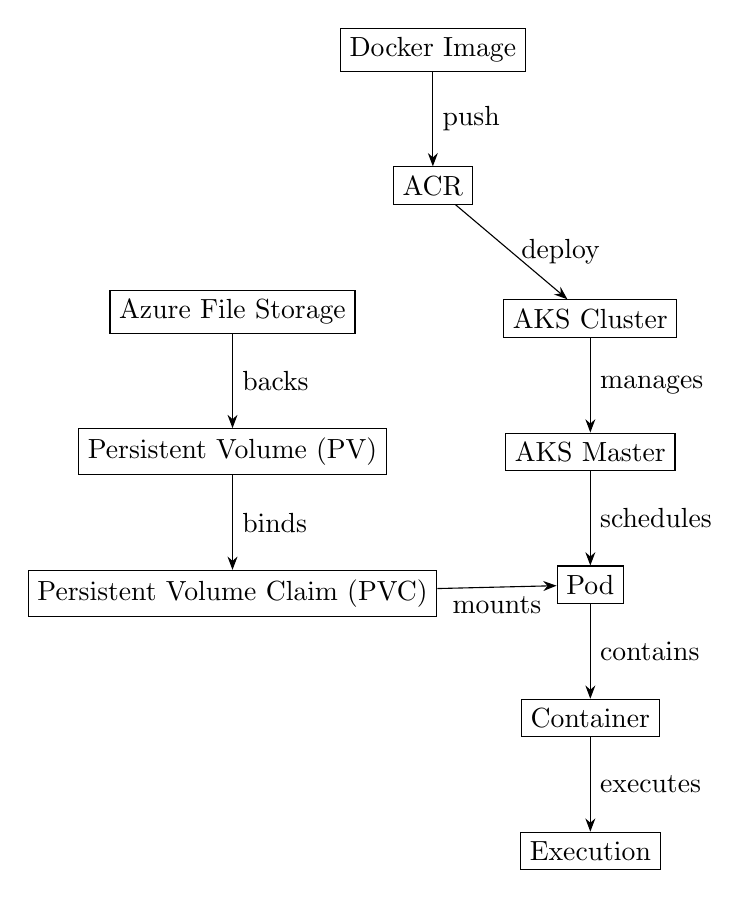
\begin{tikzpicture}[>=Stealth, node distance=1.2cm and 1.5cm]
    % Nodes
    \node (docker) [draw, rectangle] {Docker Image}; % The Docker image of your application
    \node (acr) [draw, rectangle, below=of docker] {ACR}; % Azure Container Registry where the image is stored
    \node (akscluster) [draw, rectangle, below=of acr, xshift=2cm] {AKS Cluster}; % The AKS cluster that orchestrates container deployment
    \node (aks) [draw, rectangle, below=of akscluster] {AKS Master}; % The AKS service that manages the lifecycle of containers
    \node (pv) [draw, rectangle, left=of aks] {Persistent Volume (PV)}; % Persistent storage that outlives pod lifecycles
    \node (pvc) [draw, rectangle, below=of pv] {Persistent Volume Claim (PVC)}; % A request for storage by a user
    \node (pod) [draw, rectangle, below=of aks] {Pod}; % The smallest deployable unit in Kubernetes
    \node (container) [draw, rectangle, below=of pod] {Container}; % The container that runs your application
    \node (execution) [draw, rectangle, below=of container] {Execution}; % The actual running of your application
    \node (datastore) [draw, rectangle, above=of pv] {Azure File Storage}; % Azure File Storage providing the persistent volume

    % Arrows and Annotations
    \draw[->] (docker) -- (acr) node[midway, right] {push}; % Image is pushed to ACR
    \draw[->] (acr) -- (akscluster) node[midway, right] {deploy}; % Image is deployed to AKS Cluster
    \draw[->] (akscluster) -- (aks) node[midway, right] {manages}; % AKS Service manages the deployment
    \draw[->] (aks) -- (pod) node[midway, right] {schedules}; % AKS Service schedules the pod
    \draw[->] (pv) -- (pvc) node[midway, right] {binds}; % PV is bound to PVC
    \draw[->] (pvc) -- (pod) node[midway, below] {mounts}; % PVC is mounted to the pod
    \draw[->] (pod) -- (container) node[midway, right] {contains}; % Pod contains the container
    \draw[->] (container) -- (execution) node[midway, right] {executes}; % Container executes the application
    \draw[->] (datastore) -- (pv) node[midway, right] {backs}; % Azure File Storage backs the PV
\end{tikzpicture}
\caption{General pipeline}
\label{fig:pipeline}
\end{center}
\end{figure}




\section{AKS Cluster} \index{AKS Cluster}

\subsection{Prerequisites and Description}

Before starting, ensure you have the Azure CLI installed and are logged into your Azure account. You will also need Docker installed on your local machine to create and push a container image.

\begin{figure}[H]
\includegraphics[scale=.63]{figures/aks-node-resource-interactions.png}
\caption{The diagram depicts the architecture and components involved in a Kubernetes node hosted on an Azure VM within AKS cluster. Source: MS Azure}
\label{fig:aks_node}
\end{figure}

Figure \ref{fig:aks_node} depicts the way the node in AKS operates. The Azure VM acts as the node, which is part of an Azure virtual network, and is interfaced through the Azure virtual network interface.   The node contains several key components:

\begin{description}
\item[\texttt{kubelet}]: This is the primary node agent that communicates with the Kubernetes control plane, managing the state of containers on the VM as per the desired specifications. \index{\texttt{kubelet}}

\item[Container runtime]: It is the underlying software that is used to run containers. The kubelet interacts with the container runtime to control the lifecycle of the containers.

\item[kube-proxy]: This component maintains network rules on the node, allowing for network communication to the containers from within or outside of the Kubernetes cluster.

\item[Container]: The containers run the application workloads. Each container is an isolated environment that includes the application and its dependencies. \index{Container}

\item[Azure Disk]: This represents the persistent storage option for stateful applications that require data to be retained across container restarts or node redeployments. \index{Azure Disk}

\item[Azure Files]: This is another storage option that can be used for shared storage scenarios and can be accessed by containers running in AKS. \index{Azure Files}
\end{description} 


\subsection{Setup Azure CLI and Create Resource Group}

The commands provided in this section outline the process for setting up an AKS cluster, including the registration for Windows container support and the management of node pools. These steps form the basis for deploying scalable and secure containerized applications on Azure.


Figure \ref{fig:arm} \cite{arm} illustrates the Azure Resource Manager (ARM) as the central service in Azure's architecture for managing the lifecycle of various resources like Data Stores, Web Apps, Virtual Machines, and more. Different interfaces such as the Azure portal, Azure PowerShell, Azure CLI, and REST clients interact with ARM via SDKs to perform resource management tasks, with all actions authenticated for security. ARM provides a unified and programmatic approach to deploying, managing, and monitoring Azure resources.

\begin{figure}[H]
\begin{center}
\includegraphics[scale = .45]{figures/arg.png}
\caption{Azure Resource Manager \cite{arm}}
\label{fig:arm}
\end{center}
\end{figure}

First, log into Azure and create a new resource group. Resource groups help organize your Azure resources.

\begin{lstlisting}[language=bash]
az login
az group create --name MYResourceGroup --location francecentral
\end{lstlisting}

\subsection{Create Azure Container Registry} \index{Azure Container Registry} \index{ACR}

Create an ACR \cite{acrm} to store Docker images. ACR allows you to build, store, and manage images for all types of container deployments.


Figure \ref{fig:acr} showcases the workflow of deploying a Docker container using Azure services. We start with a Local PC, where a Docker image is created. This image is then pushed to the ACR, a private repository for managing and storing Docker container images. Finally, the Docker image can be pulled from ACR to Azure Container Instances (ACI), which is a service that allows you to run containers directly on the Azure cloud, without needing to manage virtual machines or additional services. 

\begin{figure}[H] 
\begin{center}
\includegraphics[scale = .4]{figures/acr.png}
\caption{Azure Container Registry pipeline.}
\label{fig:acr}
\end{center}
\end{figure}

\begin{lstlisting}[language=bash]
az acr create --resource-group MYResourceGroup --name your-registry-name --sku Basic --admin-enabled true
\end{lstlisting}

Replace \texttt{MYResourceGroup} with the name of actual resoource group.



\subsection{Setting up AKS Cluster and Node Pools} \index{Node Pools} \index{AKS Cluster}

\subsubsection{Deploy AKS Cluster}

First, create an AKS cluster named \texttt{kubermy} within the resource group \texttt{MYResourceGroup}. This cluster will be the foundation for deploying containerized applications. Monitoring addons are enabled to provide insights into the cluster's performance, and \texttt{SSH keys} are generated for secure access. \index{\texttt{SSH keys}}

\begin{lstlisting}[language=bash]
az aks create `
    --resource-group MYResourceGroup `
    --name kubermy `
    --node-count 1 `
    --enable-addons monitoring `
    --kubernetes-version 1.27.7 `
    --generate-ssh-keys `
    --location francecentral
\end{lstlisting}

\subsubsection{Enable Windows Preview}

Before adding a Windows node pool, enable the Windows preview feature for AKS. This is necessary for clusters that will host Windows containers.

\begin{lstlisting}[language=bash]
az feature register --name WindowsPreview --namespace Microsoft.ContainerService
az provider register -n Microsoft.ContainerService
\end{lstlisting}

\subsection{Add Node Pools} \index{Node Pools}

\subsubsection{Windows Node Pool}

Add a Windows node pool named \texttt{winnp} to your AKS cluster. This node pool will allow you to deploy Windows containers alongside Linux containers in the same Kubernetes cluster.

\begin{lstlisting}[language=bash]
az aks nodepool add `
    --resource-group MYResourceGroup `
    --cluster-name myAKSCluster `
    --os-type Windows `
    --name winnp `
    --node-count 1 `
    --node-vm-size Standard_D16s_v3
\end{lstlisting}

Replace \texttt{myAKSCluster} with the name of actual AKS cluster.

More details in about node vm \texttt{Standard\_D16s\_v3} can be found in Appendix \ref{AVM}.

\subsubsection{Deleting Node Pools}

To demonstrate node pool management, the following command deletes an example Windows node pool named \texttt{winnp}. Adjust the command as necessary for your specific deployment requirements.

\begin{lstlisting}[language=bash]
az aks nodepool delete `
    --resource-group MYResourceGroup `
    --cluster-name myAKSCluster `
    --name winnp
\end{lstlisting}

\subsection{Delete AKS Cluster} \index{AKS Cluster}

For completeness, the following command illustrates how to delete the AKS cluster named \texttt{myAKSCluster}. Use this command with caution, as it will remove all resources associated with the cluster.

\begin{lstlisting}[language=bash]
az aks delete --name myAKSCluster --resource-group MYResourceGroup --yes --no-wait
\end{lstlisting}

\section{Azure Storage and Azure share file} \index{Azure Storage} \index{Azure share file}

\subsection{Azure Storage}

Figure \ref{fig:azstorage} shows four primary types of Azure Storage, that include:

\begin{description}
\item[Blob Storage]: Optimized for storing massive amounts of unstructured data, such as text or binary data, Blob Storage is ideal for serving images or documents directly to a browser, storing files for distributed access, and streaming video and audio. It can be mounted as a file system on Linux, allowing for seamless integration with Linux-based applications and services. However, \textit{it is not natively mountable on Windows machines}.

\item[File Storage]: Provides shared storage for applications using the standard SMB protocol. It is ideal for lift-and-shift applications, and for sharing files across cloud and on-premises deployments. It allows to \textit{mount directly on Windows VMs}.

\item[Queue Storage]: Supports messaging for workflow processing and for communication between components of cloud services.

\item[Table Storage]: Offers highly available, massively scalable storage, that is ideal for applications requiring a broad, flat namespace that stores structured, non-relational data.
\end{description}


\begin{figure}[H]
\begin{center}
\includegraphics[scale = .25]{figures/storage_types.png}
\caption{Storage types in Microsoft Azure Storage.}
\label{fig:azstorage}
\end{center}
\end{figure}

\subsection{Azure share file} \index{Azure} \index{Azure share file}
Azure File Share \cite{azurestorage} provides a scalable and easily accessible file storage system that integrates seamlessly with cloud and on-premises architectures. In Kubernetes environments, especially for applications requiring access to a shared file system or maintaining state across pod restarts or scaling, persistent storage is crucial. Without it, data stored within a pod would be lost upon termination or failure, leading to data loss and inconsistency. 

Figure \ref{fig:storarch} shows the Cluster Master with the API Server managing the storage resources, where a PV is provisioned from Azure Managed Disk or Azure Files. This PV is then claimed by a PVC from a Pod running on a Node within the AKS cluster, allowing the Pod to access and utilize the persistent storage as needed for stateful applications.

\begin{figure}[H]
\begin{center}
\includegraphics[scale = .7]{figures/aks-storage-options.png}
\caption{The storage architecture within an AKS cluster.}
\label{fig:storarch}
\end{center}
\end{figure}

\subsection*{Steps}

\begin{enumerate}
    \item \textbf{Create Azure Storage Account}:
    \begin{lstlisting}[language=bash]
    az storage account create --name mystorage --resource-group MYResourceGroup --location francecentral --sku Standard_LRS
    \end{lstlisting}

where \texttt{Standard\_LRS} (Standard Locally Redundant Storage) in Azure ensures that your data is replicated three times within a single storage cluster in a single data center in the same region.   
    
Replace \texttt{mystorage} with the name of actual storage.  
  
    \item \textbf{Create Azure File Share of size 100GB}:
    \begin{lstlisting}[language=bash]
    az storage share create --name myfileshare --account-name mystorage --quota 100
    \end{lstlisting}
  Replace \texttt{myfileshare} with the name of actual fileshare.  
    \item \textbf{Retrieve Storage Account Key}:
    \begin{lstlisting}[language=bash]
    STORAGE_KEY=$(az storage account keys list --resource-group MYResourceGroup --account-name mystorage --query "[0].value" -o tsv)
    \end{lstlisting}
    
    \item \textbf{Create Kubernetes Secret}:
    \begin{lstlisting}[language=bash]
    kubectl create secret generic azure-secret --from-literal=azurestorageaccountname=mystorage --from-literal=azurestorageaccountkey=$STORAGE_KEY
    \end{lstlisting}
    
    \item \textbf{Deploy PV and PVC}. Detailed YAML manifest configurations can be found in Appendix \ref{pvc} and \ref{pv}:
    \begin{lstlisting}[language=bash]
    kubectl apply -f azurefile-pv.yaml
    kubectl apply -f azurefile-pvc.yaml
    \end{lstlisting}
    
    \item \textbf{Verify PVC Binding}:
    \begin{lstlisting}[language=bash]
    kubectl get pvc azurefile
    \end{lstlisting}
    
    \item \textbf{Force Delete PVC (If Needed)}:
    \begin{lstlisting}[language=bash]
    kubectl patch pvc azurefile -p "{\"metadata\":{\"finalizers\":[]}}"
    \end{lstlisting}
\end{enumerate}

\subsection{Access to Azure File Share}

In order to have access to Azure File Storage you need Access keys.
Retrieve the keys.
\begin{lstlisting}[language=bash]
az storage account keys list --account-name mystorage --output table
\end{lstlisting}
\begin{itemize}
\item Choose a key to use: You can use either of these keys to access your Azure File Share. 
\item On your Windows system, open 'File Explorer'. Right-click on 'This PC' and choose 'Map network drive'. 
\item Select a drive letter of your choice. For the folder, enter the file share path in the format: \texttt{\\ mystorage.file.core.windows.net\textbackslash myfileshare}
\item  When prompted, enter the storage account name as the username. Use the key value copied earlier as the password.
\end{itemize}

\section{Application Deployment} \index{Deployment}
\subsection{Prepare Application for Deployment}

Build your Docker image \cite{dockerbuild} and push it to the ACR. Replace \texttt{your-registry-name} with your ACR name. Make sure that the \texttt{.Dockerfile} \index{\texttt{.Dockerfile}} is ready, an example can be found in Appendix \ref{dockerfile}.

\begin{lstlisting}[language=bash]
docker build -t your-registry-name.azurecr.io/my-app:latest .
az acr login --name your-registry-name
docker push your-registry-name.azurecr.io/my-app:latest
\end{lstlisting}

The script shows how to build a Docker image, log in to ACR, and push the image to the ACR \index{ACR}. First, it builds a Docker image named \texttt{my-app:latest} from the current directory. Second, it logs into an ACR specified by \texttt{your-registry-name}, and then pushes the newly created image to the same ACR.  The \texttt{-t} flag tags the built image with the name \texttt{your-registry-name.azurecr.io/my-app} and the tag \texttt{latest}. In particular, \texttt{your-registry-name.azurecr.io} typically refers to the address of a specific container registry (in this case, ACR) This process insures that the Docker images are stored in Azure, making them accessible for deployment in cloud environments. \index{ACR} \index{Docker}

We can list all ACRs in the Azure's subscription.
\begin{lstlisting}[language=bash]
az acr list --output table
az acr list --resource-group [ResourceGroupName] --output table
\end{lstlisting}

\subsection{Deploy Application} \index{Deployment}

 
kubectl is the command line tool for interacting with Kubernetes clusters. Kubernetes, often abbreviated as K8s, is an open-source platform designed to automate deploying, scaling, and operating application containers.

\begin{enumerate}
    \item Deploy the application to AKS using a deployment configuration file. This creates a pod running your application. More details on \texttt{YAML} manifest configuration can be found in Appendix \ref{deploy}. \index{AKS} \index{\texttt{YAML}}
    
    \begin{lstlisting}[language=bash]
    kubectl apply -f deployment.yaml
    \end{lstlisting}
    
    \item Verify the deployment and watch the pod's status to ensure the application runs correctly. 
    \begin{lstlisting}[language=bash]
    kubectl get deployment my-app-deployment
    kubectl get pods -l app=my-app --watch
    \end{lstlisting}
where \texttt{-l} means to filter the list of pods to only show those with a label \texttt{app} that has the value \texttt{my-app}.   And the flag \texttt{-watch} is used to continuously monitor the state of the specified resources in real-time.
  
 The name of deployment corresponds to the name define in the \texttt{YAML} manifest, see in Appendix \ref{deploy}. It can also be found in CLI:
     \begin{lstlisting}[language=bash]
    kubectl get deployments
    \end{lstlisting}
    \item If you need to access the PowerShell within a running pod, use the following command. Replace \texttt{[your-pod-name]} with the name of your pod.
    
    \begin{lstlisting}[language=bash]
    kubectl exec -it [your-pod-name] -- powershell
    \end{lstlisting}
    
    \item Delete the deployment if necessary, or scale it down to prevent the application from restarting.
    
    \begin{lstlisting}[language=bash]
    kubectl delete deployment my-app-deployment
    kubectl scale deployment my-app-deployment --replicas=0
    \end{lstlisting}
\end{enumerate}

\subsection{Managing \texttt{cronjobs}} \index{\texttt{cronjobs}}

The \texttt{kubectl} command is used to create a \texttt{cronjob} object which, upon the scheduled time, spawns a \texttt{Job} object. This, in turn, creates one or more pods within the Kubernetes cluster to execute the tasks. Figure \ref{fig:cronjobscheme} describes the cronjob's pipeline \cite{cronjobs1}. \index{\texttt{kubectl}}

\begin{figure}[h]
\begin{center}
\includegraphics[scale = .7]{figures/Cron-Jobs1.png}
\caption{\texttt{cronjob}'s  scheme.}
\label{fig:cronjobscheme}
\end{center}
\end{figure}

Main steps to deploy and manage \texttt{cronjob}:

\begin{enumerate}
    \item Deploy \texttt{cronjob} to schedule the application tasks. The \texttt{cronjob} configuration is defined in \texttt{cronjob.yaml}. More details on \texttt{YAML} manifest configuration can be found in Appendix \ref{cronJ}.
    
    \begin{lstlisting}[language=bash]
    kubectl apply -f cronjob.yaml
    \end{lstlisting}
Apply a configuration to a resource by file name or stdin.  \texttt{-f} means filename that contains a configuration \cite{kubecommands}.   
    \item Inspect the cron job to verify its configuration and schedule.
    
    \begin{lstlisting}[language=bash]
    kubectl describe cronjob my-app-cronjob
    \end{lstlisting}
    
    \item For manual testing of the \texttt{cronjob}, create a job from the \texttt{cronjob} definition and observe its execution.
    
    \begin{lstlisting}[language=bash]
    kubectl create job --from=cronjob/my-app-cronjob test-my-job
    kubectl get job test-my-job
    kubectl get pods --selector=job-name=test-my-job
    kubectl logs <pod-name>
    kubectl delete job test-my-job
    \end{lstlisting}
Replace \texttt{myapp-cronjob} with the name of actual \texttt{cronjon}.    
    \item Retrieve AKS credentials to interact with your cluster. \index{AKS}
    
    \begin{lstlisting}[language=bash]
    az aks get-credentials --resource-group MYResourceGroup --name myAKSCluster
    \end{lstlisting}
    
    \item View all pods in wide format to check their statuses and node allocations.
    
    \begin{lstlisting}[language=bash]
    kubectl get pods -o wide
    \end{lstlisting}
where \texttt{-o wide} is used to outpute more detailed information like the node name on which each pod is running, the pod's IP address etc.    
    \item Based on the schedule defined in the \texttt{cronjob}, it will create Jobs at specific times. We can check if any Jobs have been created by \texttt{cronjob} and if a Job has been created, we can check its logs to see if it executed successfully.
    
        \begin{lstlisting}[language=bash]
    kubectl get jobs
    kubectl logs job/<job-name>
    \end{lstlisting}
\end{enumerate}



\subsection{Accessing the Application}

Execute the following command to access the PowerShell interface of the running container. Replace \texttt{[your-pod-name]} with the name of your pod.

\begin{lstlisting}[language=bash]
kubectl exec -it [your-pod-name] -- powershell
\end{lstlisting}


\subsection{Cleanup}

After testing, you can delete the deployment or scale it down to zero replicas to stop the application.

\begin{lstlisting}[language=bash]
kubectl delete deployment my-app-deployment
kubectl scale deployment my-app-deployment --replicas=0
\end{lstlisting}


\section{Managing AKS Clusters and Node Pools} \index{Node Pools} \index{AKS Clusters}

\subsection{Listing AKS Clusters}

To view all AKS clusters within your Azure subscription, use the following command. This can help you verify the existence and status of your clusters.

\begin{lstlisting}[language=bash]
az aks list --output table
\end{lstlisting}

\subsection{Managing Node Pools}

\subsubsection{Listing Node Pools}

To list all node pools associated with a specific AKS cluster, use the command below. This provides a quick overview of the resources allocated to your cluster.

\begin{lstlisting}[language=bash]
az aks nodepool list --resource-group MYResourceGroup --cluster-name myAKSCluster --output table
\end{lstlisting}

\subsubsection{Scaling Node Pools}

Adjust the number of nodes in a specific node pool to meet your application's demands. This example scales the Windows node pool to one node.

\begin{lstlisting}[language=bash]
az aks nodepool scale --resource-group MYResourceGroup --cluster-name myAKSCluster --name winnp --node-count 1
\end{lstlisting}

% Uncomment the following section if you wish to include instructions for updating the node pool's VM size.
% \subsubsection{Updating Node Pool VM Size}
%
% To change the VM size for a node pool, which can adjust the compute resources available to your applications, use this command:
%
% \begin{lstlisting}[language=bash]
% az aks nodepool update --resource-group MYResourceGroup --cluster-name kubermy --name winnp --node-vm-size Standard_D16s_v3
% \end{lstlisting}

\subsection{Inspecting Cluster Nodes}

\subsubsection{Listing Nodes}

View details about the nodes in your Kubernetes cluster directly using \texttt{kubectl}.

\begin{lstlisting}[language=bash]
kubectl get nodes -o wide
\end{lstlisting}

\subsubsection{Describing Nodes} \index{Node Pools}

For a more detailed view of a specific node, including its status, labels, and events, use the describe command.

\begin{lstlisting}[language=bash]
kubectl describe node akswinnp000000
\end{lstlisting}

\subsection{Deploying and Managing Applications}

\subsubsection{Listing Application Pods} \index{Pods}

To see the pods associated with your application, use the following label selector:

\begin{lstlisting}[language=bash]
kubectl get pods -l app=my-app
\end{lstlisting}

\subsubsection{Integrating ACR} \index{ACR} \index{AKS}

Ensure your AKS cluster can securely pull images from your ACR by updating the AKS configuration.

\begin{lstlisting}[language=bash]
az aks update -n myAKSCluster -g MYResourceGroup --attach-acr your-registry-name
\end{lstlisting}

\subsection{Troubleshooting}

\subsubsection{Checking ACR Repositories}

If you encounter issues with image pulls, verify the repositories and tags in your ACR.

\begin{lstlisting}[language=bash]
az acr repository list --name your-registry-name --output table
az acr repository show-tags --name your-registry-name --repository my-app --output table
\end{lstlisting}


\section*{Summary}

By following the steps outlined in this tutorial, you should now have a solid understanding of the process required to deploy containerized applications in AKS. From setting up the ACR to storing your Docker images, to managing persistent storage with Azure Files or Azure Managed Disks, and orchestrating these components within an AKS cluster, you are equipped to leverage the powerful capabilities of Azure for your containerized workloads.

\appendix


\section{PV and PVC in Kubernetes} \index{PV} \index{PVC}

Persistent Volumes (PVs) and Persistent Volume Claims (PVCs) \cite{azurestorage} are part of the Kubernetes storage API. They allow for storage resources to be provisioned and consumed in a way that decouples the specifics of storage from how it is used by Pods. \index{Persistent Volume} 

\subsection{PersistentVolumeClaim (PVC)} \label{pvc} \index{PVC} \index{PersistentVolumeClaim}

A PVC is a request for storage by a user. It is similar to a Pod in that Pods consume node resources and PVCs consume PV resources.

Figure \ref{fig:pers_claims} illustrates the process of implementing persistent storage in an AKS cluster. It shows how Azure Managed Disks (available in Premium or Standard storage tiers) and Azure Files (also in Premium or Standard tiers) serve as the underlying persistent storage for a PV in AKS. A PVC is issued by a user or a Kubernetes process, which is then matched with a PV by AKS based on the defined Storage Class. The PVC is used by a Pod running on a Node within the AKS cluster, allowing the Pod to access the persistent storage for its data needs.

\begin{figure}[H]
\includegraphics[scale=.6]{figures/persistent-volume-claims}
\caption{Persistent Storage in AKS}
\label{fig:pers_claims}
\end{figure}

The following \texttt{YAML} manifest allows to create a PVC on AKS. \index{\texttt{YAML}}

\begin{lstlisting}[language=yaml]
apiVersion: v1
kind: PersistentVolumeClaim
metadata:
  name: azurefile
spec:
  accessModes:
    - ReadWriteMany  # Can be mounted by multiple nodes
  storageClassName: ""  # Empty to use the default StorageClass
  resources:
    requests:
      storage: 100Gi  # Request 100 GB of storage
  volumeName: azurefile-pv  # Binds to a specific PersistentVolume
\end{lstlisting}

\begin{itemize}
    \item \texttt{accessModes}: Describes how the volume can be accessed. \texttt{ReadWriteMany} means the volume can be mounted as read-write by many nodes.
    \item \texttt{storageClassName}: Specifies the StorageClass to be used. Leaving it empty means the default StorageClass is used.
    \item \textbf{resources.requests.storage}: The amount of storage requested.
    \item \texttt{volumeName}: Specifies the binding to a specific PV. This is usually not required unless binding to a pre-provisioned PV.
\end{itemize}

\subsection{PersistentVolume (PV)} \label{pv} \index{PV} \index{PersistentVolume} \index{\texttt{YAML}}

A PV is a piece of storage in the cluster that has been provisioned by an administrator or dynamically provisioned using Storage Classes. In \texttt{YAML} manifest replace \texttt{myfileshare} with the name of actual file share.

\begin{lstlisting}[language=yaml]
apiVersion: v1
kind: PersistentVolume
metadata:
  name: azurefile-pv
spec:
  capacity:
    storage: 100Gi  # Total capacity of the PV
  accessModes:
    - ReadWriteMany  # Matches the access mode in PVC
  persistentVolumeReclaimPolicy: Retain  # Data is retained even after PVC is deleted
  azureFile:
    secretName: azure-file-secret  # Secret containing Azure storage account info
    shareName: myfileshare  # The name of the Azure File Share
    readOnly: false  # The volume can be mounted as read-write
\end{lstlisting}

\begin{itemize}
    \item \textbf{capacity.storage}: The amount of storage available on this PV. It should match or exceed the size requested in the PVC.
    \item \texttt{persistentVolumeReclaimPolicy}: Defines what happens to the PV data after the PVC is released. \texttt{Retain} keeps the data on the volume.
    \item \texttt{azureFile}: Specifies the Azure File Storage configuration.
    \item \texttt{secretName}: The name of the Kubernetes secret that contains the Azure storage account name and key.
    \item \texttt{shareName}: The name of the Azure file share.
    \item \texttt{readOnly}: Indicates whether the file share is read-only or read-write.
\end{itemize}


\section{\texttt{cronjob} Configuration in Kubernetes}

A \texttt{cronjob} \cite{cronjob} in Kubernetes is used to run jobs on a time-based schedule, similar to the cron utility in Unix-like operating systems. The following YAML configuration defines a CronJob to run a containerized application on a schedule.

\subsection{\texttt{cronjob}} \label{cronJ} \index{\texttt{cronjob}} \index{\texttt{YAML}}

The cron format is a simple, yet powerful scheduling syntax used to configure the time and frequency at which jobs are executed in a Unix-like operating system. The format consists of five fields that Cron converts into a set of time intervals.

\begin{lstlisting}
*    *    *    *    *  command to be executed
-    -    -    -    -
|    |    |    |    |
|    |    |    |    +----- day of week (0 - 7) (0 or 7 is Sun, or use names)
|    |    |    +------- month (1 - 12)
|    |    +--------- day of month (1 - 31)
|    +----------- hour (0 - 23)
+------------- min (0 - 59)
\end{lstlisting}

\begin{itemize}
    \item The first field represents the minute and accepts values from 0 to 59.
    \item The second field represents the hour and accepts values from 0 to 23.
    \item The third field is the day of the month, which accepts values from 1 to 31.
    \item The fourth field is the month of the year, accepting values from 1 to 12 or the short names of the months (e.g., `Jan`, `Feb`, `Mar`, etc.).
    \item The fifth field is the day of the week, accepting values from 0 to 7, where both 0 and 7 represent Sunday. Alternatively, you can use the short names of the days (e.g., `Sun`, `Mon`, `Tue`, etc.).
\end{itemize}

Each field can have a single value, a list of values, a range of values, or a wildcard \texttt{*}, which represents all possible values for that field. For example, a cron schedule of \texttt{0 11 * * Mon,Wed-Fri} means the job will run at 11:00 AM on Monday, Wednesday, Thursday, and Friday. In the \texttt{YAML} below replace \texttt{my-app-cronjob}, \texttt{my-app}, \texttt{my-volume}, \texttt{your-registry-name} with corresponding actual names.


\begin{lstlisting}[language=yaml]
apiVersion: batch/v1
kind: CronJob
metadata:
  name: my-app-cronjob
spec:
  schedule: "0 11 * * 1,3-5"  # At 11:00 on Monday, Wednesday, Thursday, and Friday
  jobTemplate:            # Template for the job to be run
    spec:
      template:
        spec:
          nodeSelector:
            "kubernetes.io/os": windows  # Ensure the job runs on a Windows node
          containers:
          - name: my-app
            image: your-registry-name.azurecr.io/my-app:latest  # Container image to use
            resources:
              requests:
                memory: "48Gi"  # Memory request for the container
                cpu: "12"       # CPU request for the container
            volumeMounts:
            - name: my-volume
              mountPath: "/data"  # Mount path for the volume inside the container
          volumes:
          - name: my-volume
            persistentVolumeClaim:
              claimName: azurefile  # PVC that the CronJob will use
          restartPolicy: OnFailure  # Job restart policy
\end{lstlisting}

\begin{itemize}
    \item \texttt{schedule}: Specifies when the job should be run using the Cron format.
    \item \texttt{nodeSelector}: Ensures that the job is scheduled on nodes with the specified label, in this case, Windows nodes.
    \item \textbf{containers.image}: Defines which container image should be run.
    \item \textbf{resources.requests}: Specifies the computational resources required for the container. Here it requests 48 GiB of memory and 12 CPU units.
    \item \texttt{volumeMounts}: Defines the volumes to be mounted into the containers and their mount paths.
    \item \textbf{volumes.persistentVolumeClaim}: Links the volume defined in the pod to the PVC which provides the actual storage.
    \item \texttt{restartPolicy}: The policy to apply when a job fails. \texttt{OnFailure} means the job will be retried until it succeeds.
\end{itemize}

This \texttt{cronjob} is configured to run the \texttt{my-app} container daily at 11:00 AM, ensuring it has access to the required CPU and memory resources and storage volume.

\section{Kubernetes Deployment Configuration} \index{Deployment} \index{\texttt{YAML}}

A Deployment in Kubernetes \cite{aksdeploy} is used to declare replicas of pods to run in your cluster. The following YAML configuration specifies the deployment details for the application.

\subsection{Deployment} \label{deploy}

In the \texttt{YAML} below replace \texttt{my-app-deployment}, \texttt{my-app}, \texttt{my-volume}, \texttt{your-registry-name} with corresponding actual names. \index{\texttt{YAML}}
 
\begin{lstlisting}[language=yaml]
apiVersion: apps/v1
kind: Deployment
metadata:
  name: my-app-deployment  # Name of the deployment
spec:
  replicas: 1  # Number of replicas to run
  selector:
    matchLabels:
      app: my-app  # Label selector to identify the pods
  template:  # Template for the pods
    metadata:
      labels:
        app: my-app  # Labels assigned to the pods
    spec:
      nodeSelector:
        "kubernetes.io/os": windows  # Run the pods on Windows nodes
      containers:
      - name: my-app
        image: your-registry-name.azurecr.io/my-app:latest  # Container image to deploy
        resources:
          requests:
            memory: "48Gi"  # Memory request for the container
            cpu: "12"       # CPU request for the container
        volumeMounts:
        - name: my-volume
          mountPath: "/data"  # Mount path for the volume inside the container
      volumes:
      - name: my-volume
        persistentVolumeClaim:
          claimName: azurefile  # PVC that the deployment will use
\end{lstlisting}

\begin{itemize}
    \item \texttt{replicas}: Defines the number of instances of the pod that should be running.
    \item \textbf{selector.matchLabels}: Determines how the Deployment finds which pods to manage.
    \item \textbf{template.metadata.labels}: Provides the labels for the pods that will be created.
    \item \texttt{nodeSelector}: Ensures the pods are scheduled on nodes with specific labels, in this case, Windows nodes.
    \item \textbf{containers.image}: Specifies which image should be used for creating the containers.
    \item \textbf{resources.requests}: Indicates the minimum amount of resources the container should have.
    \item \texttt{volumeMounts}: Configures the mounting of a volume within the container.
    \item \textbf{volumes.persistentVolumeClaim}: Connects a persistent volume claim (which provides persistent storage) to the pods.
\end{itemize}

This deployment configuration ensures that a single instance of the \texttt{my-app} container is running, with the required resources and storage volume, on a Windows node within your Kubernetes cluster.


\section{Integration into Github Actions} \index{Github Actions}

The description of the GitHub Actions workflow for deploying to AKS with Windows Containers \cite{Github}, \cite{Github1}. 

In the \texttt{YAML} below replace \texttt{myAKSCluster}, \texttt{myResourceGroup}, \texttt{myapp}, \texttt{your-registry-name} with corresponding actual names and \texttt{./path/to/cronjob.yaml} with actual path.

\begin{lstlisting}
name: Deploy to AKS with Windows Containers

on:
  push:
    branches:
      - main

jobs:
  build-and-deploy:
    runs-on: windows-latest

    steps:
      - name: Checkout code
        uses: actions/checkout@v2

      - name: Login to Azure
        uses: azure/login@v1
        with:
          creds: ${{ secrets.AZURE_CREDENTIALS }}

      - name: Build and push Docker image
        run: |
          docker build -t ${{ secrets.REGISTRY_LOGIN_SERVER }}/myapp:latest -f ./Dockerfile .
          docker login ${{ secrets.REGISTRY_LOGIN_SERVER }} -u ${{ secrets.REGISTRY_USERNAME }} -p ${{ secrets.REGISTRY_PASSWORD }}
          docker push ${{ secrets.REGISTRY_LOGIN_SERVER }}/myapp:latest

      - name: Set Kubernetes context
        uses: azure/aks-set-context@v1
        with:
          creds: ${{ secrets.AZURE_CREDENTIALS }}
          cluster-name: myAKSCluster
          resource-group: myResourceGroup

      - name: Deploy CronJob to AKS
        run: |
          kubectl apply -f ./path/to/cronjob.yaml
\end{lstlisting}


\textbf{Workflow Name}: \texttt{name: Deploy to AKS with Windows Containers}
\begin{itemize}
    \item Specifies the name of the workflow, serving as a label for identification in the GitHub Actions UI.
\end{itemize}

\textbf{Trigger}: \texttt{on: push: branches: - main}
\begin{itemize}
    \item Defines when the workflow should be triggered, configured to run on pushes to the \texttt{main} branch of the repository.
\end{itemize}

\textbf{Job Definition}: \texttt{jobs: build-and-deploy: runs-on: windows-latest}
\begin{itemize}
    \item Defines a job named \texttt{build-and-deploy}.
    \item Specifies that the job should run on a Windows-based runner (\texttt{windows-latest}).
\end{itemize}

\textbf{Steps}:
\begin{enumerate}
    \item \textbf{Checkout Code}: 
    \begin{itemize}
        \item Uses the \texttt{actions/checkout@v2} action to check out the repository code into the GitHub runner.
    \end{itemize}
    \item \textbf{Login to Azure}:
    \begin{itemize}
        \item Utilizes the \texttt{azure/login@v1} action for Azure authentication, requiring the
        
         \texttt{AZURE\_CREDENTIALS} secret with Azure Service Principal JSON credentials.
    \end{itemize}
    \item \textbf{Build and Push Docker Image}:
    \begin{itemize}
        \item Builds the Docker image from the Dockerfile and pushes it to the ACR.
    \end{itemize}
    \item \textbf{Set Kubernetes Context}:
    \begin{itemize}
        \item Employs the \texttt{azure/aks-set-context@v1} action to set the Kubernetes context for the specified AKS cluster and resource group.
    \end{itemize}
    \item \textbf{Deploy CronJob to AKS}:
    \begin{itemize}
        \item Executes \texttt{kubectl apply} to deploy the CronJob to the AKS cluster, with the path 

\texttt{./path/to/your/cronjob.yaml} replaced by the actual path to the CronJob YAML file in the repository.
    \end{itemize}
\end{enumerate}

The workflow is designed to automate the deployment process to AKS, with the primary requirement being the adjustment of the path to the CronJob YAML file. The rest of the workflow utilizes predefined secrets and settings.

\section{Selection of Azure Virtual Machine} \label{AVM} \index{Virtual Machines}

The list of VMs available in Azure can be found in \cite{avm}.

In selection of VM the following factors are important:
\begin{itemize}
\item Workload Requirements: Understand the demands of the applications in terms of CPU, memory, storage, and network performance.
\item Scalability and Performance.
\item Availability of VM Sizes in Your Region: Not all VM sizes are available in every Azure region. 
\item Cost: Larger VMs are more expensive.
\end{itemize}

For example, \texttt{Standard\_D16s\_v3},  is part of the D-series Azure VMs, optimized for applications that require a balance of CPU and memory: 16 CPU cores, 64 GB of RAM and \texttt{D16s} suggests that it supports Premium SSDs.

Figure \ref{fig:price_vm} shows the pricing for \texttt{Standard\_D16s\_v3} vm.

\begin{figure}[H] 
\begin{center}
\includegraphics[scale = .3]{figures/prices_vm.png}
\caption{Prices for a \texttt{Standard\_D16s\_v3} vm}
\label{fig:price_vm}
\end{center}
\end{figure}


\section{Azure Storage Selection} \index{Azure Storage}
Figure \ref{fig:price_ss} shows the prices for different options of storage. 

\begin{figure}[H] 
\begin{center}
\includegraphics[scale = .45]{figures/price_storage.png}
\caption{Prices in Azure Files}
\label{fig:price_ss}
\end{center}
\end{figure}

The code below allows you to extract the information about file storage account.

    \begin{lstlisting}[language=bash]
    az storage account list --output table
    az storage share list --account-name [StorageAccountName] --output table
    az storage share show --name [ShareName] --account-name [StorageAccountName]
    \end{lstlisting}

In the output, we see that the size of the file share is set to 100 GB and \texttt{AccessTier:}

 \texttt{"TransactionOptimized"} shows that  "TransactionOptimized" performance tier is chosen.
    
    \begin{lstlisting}    
{
  "accessTier": "TransactionOptimized",
  "deleted": null,
  "deletedTime": null,
  "lease": {
    "duration": null,
    "state": "available",
    "status": "unlocked"
  },
  "metadata": {},
  "name": "myfileshare",
  "nextAllowedQuotaDowngradeTime": null,
  "properties": {
    "etag": "\"0x8DC29BBDD441DBD\"",
    "lastModified": "2024-02-09T22:10:02+00:00",
    "quota": 100
  },
  "protocols": null,
  "provisionedBandwidth": null,
  "provisionedEgressMbps": null,
  "provisionedIngressMbps": null,
  "provisionedIops": null,
  "remainingRetentionDays": null,
  "rootSquash": null,
  "snapshot": null,
  "version": null
}    
\end{lstlisting}

More details can be found in \cite{storageprice} and \cite{azurebills}.


\section{Dockerfile manifest} \label{dockerfile} \index{\texttt{.Dockerfile}}

This \texttt{.Dockerfile} is designed for creating a Windows-based Docker image that sets up a Python development environment with Git, and is tailored for deploying a Python application.

\begin{lstlisting}[language=yaml]
# Use a Windows base image
ARG GITHUB_TOKEN

FROM mcr.microsoft.com/windows/servercore:ltsc2022

# Set the working directory in the container
WORKDIR C:\\myapp

# Use PowerShell for subsequent commands
SHELL ["powershell", "-Command", "$ErrorActionPreference = 'Stop';"]

# Install Python and Git
# Note: Replace the URLs with the actual URLs for Python and Git installers
RUN Invoke-WebRequest -Uri 'https://www.python.org/ftp/python/3.9.0/python-3.9.0-amd64.exe' -OutFile 'python_installer.exe' -UseBasicParsing; \
    Start-Process python_installer.exe -ArgumentList '/quiet InstallAllUsers=1 PrependPath=1' -Wait; \
    Remove-Item python_installer.exe -Force; \
    Invoke-WebRequest -Uri 'https://github.com/git-for-windows/git/releases/download/v2.28.0.windows.1/Git-2.28.0-64-bit.exe' -OutFile 'git_installer.exe' -UseBasicParsing; \
    Start-Process git_installer.exe -ArgumentList '/VERYSILENT /NORESTART /NOCANCEL /SP-' -Wait; \
    Remove-Item git_installer.exe -Force
    # Invoke-WebRequest -Uri 'https://curl.se/ca/cacert.pem' -OutFile 'cacert.pem'; \
    # [System.Environment]::SetEnvironmentVariable('GIT_SSL_CAINFO', 'C:\codpy\cacert.pem', [System.EnvironmentVariableTarget]::Machine); \
    # Remove-Item cacert.pem -Force

# Add Python and Git to PATH (replace with the actual installation paths if different)
RUN $env:Path += ';C:\\Program Files\\Python39;C:\\Program Files\\Python39\\Scripts;C:\\Program Files\\Git\\cmd'; \
    [Environment]::SetEnvironmentVariable('Path', $env:Path, [EnvironmentVariableTarget]::Machine)

# Set the GitHub token as an environment variable
ENV GITHUB_TOKEN=$GITHUB_TOKEN

# Use the token to install the codpy package from the private repository
RUN $Env:GITHUB_TOKEN='YOURGITHUBTOKEN'; \
    git clone https://yourrepo:$Env:GITHUB_TOKEN@github.com/yourrepo/myapp.git; \
    cd myapp; \
    pip install .

# Reset the working directory to C:\app
WORKDIR C:\\app

# Copy the content of the local src directory to the working directory
COPY . C:\\app

# Install any dependencies from requirements.txt
RUN pip install --no-cache-dir -r requirements.txt

# If necessary,  copy the specific .pyd file to the site-packages directory
COPY ["yourapp.cp39-win_amd64.pyd", "C:/Program Files/Python39/Lib/site-packages/"]

# Command to run on container start
#CMD ["powershell", "-Command", "while ($true) { Start-Sleep -Seconds 3600 }"]

CMD ["python", "C:\\app\\main.py"]
\end{lstlisting}

\begin{description}
\item[Base Image]: The image starts from a Windows Server Core base image (\texttt{ltsc2022}). This provides the underlying Windows operating system environment.

\item[Working Directory]: It sets the working directory inside the container to \texttt{C:/\ myapp}, which is where subsequent commands will operate.

\item[Shell Setting]: The shell is set to PowerShell with error preferences, ensuring that subsequent commands are run using PowerShell and that any errors stop the process.

\item[Python and Git Installation]: It installs Python and Git by downloading their installers from specified URLs and running them silently. After installation, the installers are removed to keep the image size down.

\item[Path Environment Variable]: The \texttt{Dockerfile} appends the Python and Git executable paths to the system PATH environment variable, allowing these programs to be run from any location within the container.

\item[GitHub Token]: Sets an environment variable \texttt{GITHUB\_TOKEN} using the build argument \texttt{ARG GITHUB\_TOKEN}, which is intended to be used for secure access to private repositories.

\item[Clone and Install Python Application]: It uses the provided GitHub token to clone a Python application from a private GitHub repository. Then it changes to the application directory and installs it using pip. This process assumes that the application has a setup.py file for installation.

\item[Reset Working Directory]: The working directory is reset to \texttt{C:/\ app}.

\item[Copy Application Files]: Copies the application files from the local source directory to the container's working directory.

\item[Install Dependencies]: Installs any dependencies specified in requirements.txt using pip.

\item[Copy \texttt{.pyd} File]: If necessary, copies a specific \texttt{.pyd} file (a Python extension module) to the Python site-packages directory, which is where Python looks for installed packages.

\item[Set Startup Command]: Finally, it sets the default command to run the Python application (main.py) located at \texttt{C:/\ app/\ main.py} when the container starts.
\end{description}

\begin{thebibliography}{1}
\bibitem{docker} Docker's glossary. \url{https://docs.docker.com/glossary/}
\bibitem{dockerbuild} \href{https://docs.docker.com/engine/reference/commandline/image_build/}{docker build (docker image build)}
\bibitem{docker_use} \href{https://www.docker.com/resources/what-container/}{Use containers to Build, Share and Run your applications}
\bibitem{azure}\href{https://learn.microsoft.com/en-us/azure/azure-glossary-cloud-terminology}{Microsoft Azure' glossary}. 
\bibitem{kuber} \href{https://www.bluematador.com/learn/kubernetes-glossary}{Kubernetes' glossary}.
\bibitem{kubazure} \href{https://learn.microsoft.com/en-us/azure/aks/concepts-clusters-workloads}{Core Kubernetes concepts for Azure Kubernetes Service} 
\bibitem{cronjob} \href{https://learn.microsoft.com/en-us/azure/azure-functions/functions-bindings-timer?tabs=python-v2\%2Cisolated-process\%2Cnodejs-v4&pivots=programming-language-powershell}{Timer trigger for Azure Functions}
\bibitem{kupv} \href{https://kubernetes.io/docs/concepts/storage/persistent-volumes/}{Persistent Volumes on Kubernetes}
\bibitem{azurestorage} \href{https://learn.microsoft.com/en-us/azure/aks/concepts-storage}{Storage options for applications in Azure Kubernetes Service (AKS)}
\bibitem{aksdeploy} \href{https://learn.microsoft.com/en-us/azure/aks/learn/quick-kubernetes-deploy-cli}{Quickstart: Deploy an Azure Kubernetes Service (AKS) cluster using Azure CLI}
\bibitem{acrm} \href{https://dubeyanjali1303.medium.com/azure-container-registry-part-1-c6d7271426f8}{Azure Container Registry — Part 1 | by Anjali Dubey | Medium}
\bibitem{Github} \href{https://github.com/marketplace/actions/kubernetes-action}{GitHub Action:
Kubernetes Action}
\bibitem{Github1} \href{https://github.com/marketplace/actions/deploy-to-kubernetes-cluster}{GitHub Action Deploy to Kubernetes cluster}
\bibitem{cronjobs1} \href{https://www.zenesys.com/kubernetes-cronjobs-how-to-run}{KUBERNETES CRONJOBS - HOW TO RUN CRON JOB IN KUBERNETES?}
\bibitem{kubelet} \href{https://kubernetes.io/docs/reference/command-line-tools-reference/kubelet/}{Kubernetes : kubelet}
\bibitem{arm} \href{https://learn.microsoft.com/en-us/azure/azure-resource-manager/management/overview}{What is Azure Resource Manager?}
\bibitem{smbprotocol} \href{https://en.wikipedia.org/wiki/Server_Message_Block}{Wikipedia page on: Server Message Block}
\bibitem{smb} \href{https://learn.microsoft.com/en-us/azure/storage/files/files-smb-protocol?tabs=azure-portal}{SMB file shares in Azure Files}
\bibitem{kubecommands} \href{https://kubernetes.io/docs/reference/generated/kubectl/kubectl-commands}{kubetcl commands list}
\bibitem{avm} \href{https://azure.microsoft.com/en-us/pricing/details/virtual-machines/series/}{Virtual Machine series}
\bibitem{azurebills} \href{https://learn.microsoft.com/en-us/azure/storage/files/understanding-billing}{Understand Azure Files billing}
\bibitem{storageprice} \href{https://azure.microsoft.com/en-us/pricing/details/storage/files/}{Azure Files pricing}
\bibitem{kubboot} \href{https://kubernetesbootcamp.github.io/kubernetes-bootcamp/1-1.html}{Kubernetes bootcamp}
\bibitem{kubmaster} \href{https://kubernetes.io/fr/docs/concepts/architecture/master-node-communication/}{Communication Master-Node}
\bibitem{azurecli} \href{https://learn.microsoft.com/en-us/cli/azure/}{Azure Command-Line Interface (CLI) documentation}
\bibitem{azlist} \href{https://learn.microsoft.com/en-us/cli/azure/reference-docs-index}{Azure CLI conceptual article list}
\bibitem{azurecliinstall} \href{https://learn.microsoft.com/en-us/cli/azure/install-azure-cli}{How to install the Azure CLI}
\end{thebibliography}

\printindex

\end{document}
